\documentclass{article}
\usepackage{mathtools}
\usepackage{pdfpages}
\usepackage[]{mcode}

\begin{document}
\title{Modeling Acoustic Propagation in Fluids\\}
\author{Taylor Fahlman}
\maketitle

\section{Introduction}

Sound surrounds us every day. It is important to our everyday lives; we use hearing and sound for survival,
productivity, and enjoyment. Sound is one of the most important aspects of living. Because of this, the 
understanding of sound and modeling its various properties today is important. Researchers use various
models of sound to understand more finely its characteristics. How sound propagates in fluids, specifically
water and air in most cases, can provide insight into a number of different systems. For example, modeling
acousitcs in a concert hall or similar musical venue can show engineers how best to build the room to
optimize the musical or otherwise acoustic result of the performance. Another very important example
in medicine is ultrasounds. Modeling how sound can propagate through fluids (and other mediums) enable
doctors and software engineers to accurately represent and interpret the results of an ultrasound
procedure. A third example is being able to locate objects underwater. The military uses models
of sound propagation in water to locate submarines in the ocean while on patrol. Similarly,
researchers use models of sound propagation to locate and identify whale pods. Each pod uses
a unique frequencey and patterns to communicate, a kind of pseudo-language. Understanding how
various frequencies move in different ways through water help researchers track migration patters,
proximity of pods, and various other information vital to their research. These are only a few
examples of sound modeling. There are many various fields these methods can be applied to. These
examples show the importance of sound modeling, as well as the wide range of applications it can have.

\newpage
\section{Previous Work}
Due to the wide array of applications, there are many methods to modeling sound, and each has certain
aspects it focuses on. For example, some models focus on the density of the fluid, while others factor
in temperature. There are also different methods for modeling one-dimensional, two-dimensional and
three-dimensional propagations. Also, some models only look at sound traveling through fluids, but
others look at how sound results from fluid moving. All of these various models make it difficult to 
find exact one needed for a given situation. The variability in application also means a variability 
in complexity. This means that overall, it is hard to find and compute the precise solution one wants.
Particulary for this problem, the main methods involve either the wave equation, or the Euler identity. 
Two-dimensional methods use a linear Euler, while three-dimensional use a Non-linear Euler identity, 
and the equation used measures how sound propogates through water. The model used here is two-dimensional,
linear Euler equation, focusing on the sound pressure and velocity. Only focusing on these two aspects
make the model a fast way to find a solution. However, this does not factor temperature, or a number of 
other important factors. This means that while the solution may be quick, it is more of a rough esitmate
for an actual system, and may not be suitable for measurements that need high degrees of accuracy.
However, for this analysis, it is more than adequate.

\section{Contribution}
In particular, this project is exploring the relationship between velocity and sound pressure. 
Specfically, to explore the relationship between sound pressure and how velocity affects the
propagation of various values of pressure. While the research paper (Othman) has already given a solution
for the equation, it is a general solution and the results it graphs revole around pressure. Instead,
this project aims to graph how the initial velocity affects the distance travled. A matlab script
will be written and run, using initial values given by the paper, and taking the initial value of velocity,
will graph the distance against velocity for a number of given pressures. Once all of these data points are
found, then an analysis of how the velocity affects distance will be graphed. This way we can see how velocity
and pressure are related. This information can help in analysis and understanding of sound in fluids.
If time permits, testing the same set of pressures and velocities in various fluids will be done. The first
fluid will be water, and the secondary fluid will be air, and possibly some very vicsous fluid as the third.\\

\subsection{Model}
The following system of equations is used in the final model:
\begin{equation}
    -\rho v(x,y,t) = 1/c^2(\delta p(x,y,t)/\delta t)
\end{equation}
\begin{equation}
    \delta p(x,t,y)/\delta_x = -\rho (\delta v_x(x,y,t)/\delta t)
\end{equation}
\begin{equation}
    \delta p(x,t,y)/\delta_y = -\rho (\delta v_y(x,y,t)/\delta t)
\end{equation}

Where the particle velocity is
\begin{equation}
    v(x,y,t) = xv_x(x,y,t) + yv_y(x,y,t)
\end{equation}
and the pressure is
\begin{equation}
    p(x,t,y)
\end{equation}
The density is rho, with a wave number 
\begin{equation}
    k = (\omega/c) + i\alpha
\end{equation}
where omega is the angular frequency, c is the speed of sound in the medium, and alpha is attenuation in an
inhomogeneous medium.

Using Euler's identity, these equations we get the following

\begin{equation}
    G1 = (1/2)(P* + (i\rho\omega/m)F*)
\end{equation}
\begin{equation}
    G2 = (1/2)(P* - (i\rho\omega/m)F*) 
\end{equation}
\begin{equation}
    m^2 = [k^2 - (\omega^2/c^2)]
\end{equation}
\begin{equation}
    P(x,y,t) = [G1e^{-mx} +G2e^{mx}]e^i(\omega t + ky)
\end{equation}
\begin{equation}
    V_x(x,y,t) = (m/\rho\omega)[G1(k,\omega)e^{-mx} - G2(k,\omega)e^{mx}]e^i(\omega t+ky)
\end{equation}
\begin{equation}
    V_y(x,y,t) = (-k/\rho\omega)[G1(k,\omega)e^{-mx} + G2(k,\omega)e^{mx}]e^i(\omega t+ky)
\end{equation}

\section{Prediction}

Given the wide variability of this model, the outcome is uncertain. In comparing fluids, it is known
that acoustics propgate faster/more easily in water than in air. That outcome is expected. However, for the
more viscous fliud, given that there is time to test it, I would expect it to propagate slower than water.
The reason that sound moves through water specifically faster is that is doesn't compress, as air does
when sound travels through it. However, with a viscous fluid, sound should move slower since it takes
more energy to move through a fluid as it gets more viscous. The model should reflect this with the 
alpha variable, which is the attenuation or loss of intensity in a fluid. The larger this is, the
larger the velocity must be to overcome it. The density, rho, is the main variable that represents
viscosity as well, and will also influence the outcome significantly. Perhaps the density will allow
the sound to travel faster similar to traveling through a solid. 
For the relationship between velocity and pressure, the outcome of this is also uncertain. It will be
interesting to analyze and interpret the data. Based on the current knowledge and progression of this
project, it seems as if the velocity will carry the sound further the higher it is. As well, it 
seems as if the pressure will push the sound further, as it has more energy. However, the deceleration in
certain fluids may be too high for the veloicity to overcome and there could exist some terminal velocity
where only changing the pressure can increase the distance traveled, but this model may not be complex enough
to simulate that. 
Due to the fact that the model uses a linear Euler method, the velocity and pressure are expected to have
roughly a linear relationship, with their ratio dependent on the density, speed of sound and gradient
of the pressure. The linear relationship should therefore get steeper as the viscosity increases. 
Given enough tests with various viscosities, there should be a point at which increasing the viscosity
should no longer affect the linear relationship much because it will approach an asymptote. This fluid
may not exist in real life. There should also be a fluid, most likely water, in which the relationship
is 1-to-1, or where the graph is the same as f(x) = x. Air should have a flatter slope, as velocity
should be more important than pressure since the density of air is much lower relatively. 
Overall, the linear relationship between velocity and pressure should become steeper as the density
increases, and flatter as the density decreases. It is also expected that at some point, the velocity
will stop having an affect on the distance as the viscosity of the fluid increases.

\section{MATLAB Solution} 
Using equation 12 from Section 3.1, the following MATLAB solution was implemented

\begin{lstlisting}
dens = 998; %density of water, 1.225 for air
c = 1481; %Speed of sound in water, 343 in air
freq = 50000; %frequency
w = 2*pi*freq; %Angular frequency
p0 = 1;
f0 = 1;
alpha = .0022; %Attenuation in water, 1.64 for air (from Wikipedia)
k = (w/c) + (1i*alpha); %Wave number
m = sqrt((k*w) - ((w*w)/(c*c)));
x = 1;
y = 1;
t = 10;
g1 = (.5)*(p0 + ((1i*dens*w)/(m))*f0)
g2 = (.5)*(p0 - ((1i*dens*w)/(m))*f0)

d = propfunc(x, y, t, w, m, k, g1, g2);
\end{lstlisting}
\newpage
Where propfunc is defined as
\begin{lstlisting}
function [ dist ] = p(x, y, t, w, m, k, g1, g2)

dist = (g1*exp(-m*x) + g2*exp(m*x))*exp(1i)*((w*t)+(k*y));
\end{lstlisting}

\section{Results}
Given the short amount of time to run the experiments, only water and air were able to be tested with the code.
The predictions made were correct, in that the distance traveled in air by a certain sound wave was much less
than the distance traveled by the same sound wave in water. This was mostly due to the vast difference in the
speed of sound in the respective fluids, as well as the attenuation constant inherent in those fluids. In the first figure in the appendix,
we can see the estimated distance in water of both 100 KHz and 50 KHz. Interestingly, the lower frequency seems
to travel further than the higher frequency, due to a much slower rate of decay. In the second figure, we can see that the
distance travel in air is significantly less for both 50 and 100 KHz. Unfortunately, there was no time to test other
fluids. But assuming the rest follow this general pattern, the stated predictions will most likely be accurate.


\section{Further Work}
In the future, hopefully more fluids will be tested and patterns analyzed. The model itself is also very basic;
it does not account for temperature fluctuations and pockets, viscosity changes, or other complex properties
that fluids can have. There will never be a perfect universal model, but this one could stand to be expanded.
As well, a mutli-dimensional model, using a non-linear method would probably yield more accurate and interesting
results in the end. However, this model is still useful for fast and simple calculations. Continued work on this
model would also yield benefits for 2D measurements. 

\section{Sources}
Numerical Method for Modeling of Acoustic Waves Propagation - Dykas, Wroblewski, Rulik, Chmielniak, 2010\\
Governing Equations for Wave Proagation, K. N. van Dalem 2013\\
Analytical Solution for Acoustic Waves Propagation in Fluids - Othman, Sayed Ali, Farouk, 2011\\
Wikipedia - Wave Equation\\
Wikipedia - Attenuation\\


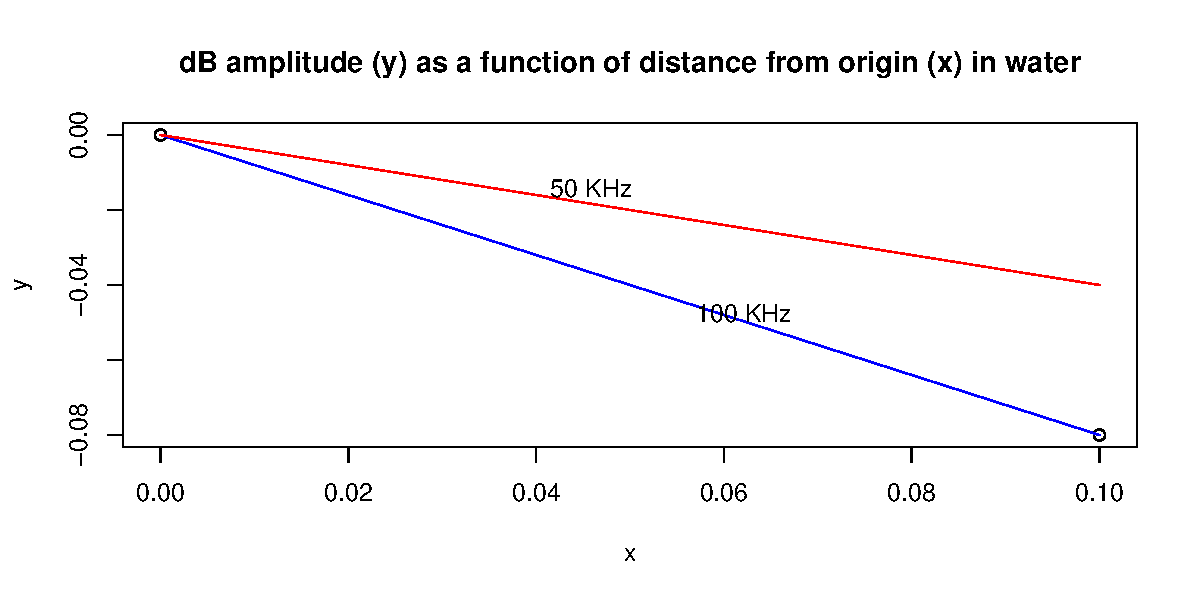
\includepdf[pages={1}]{water.pdf}
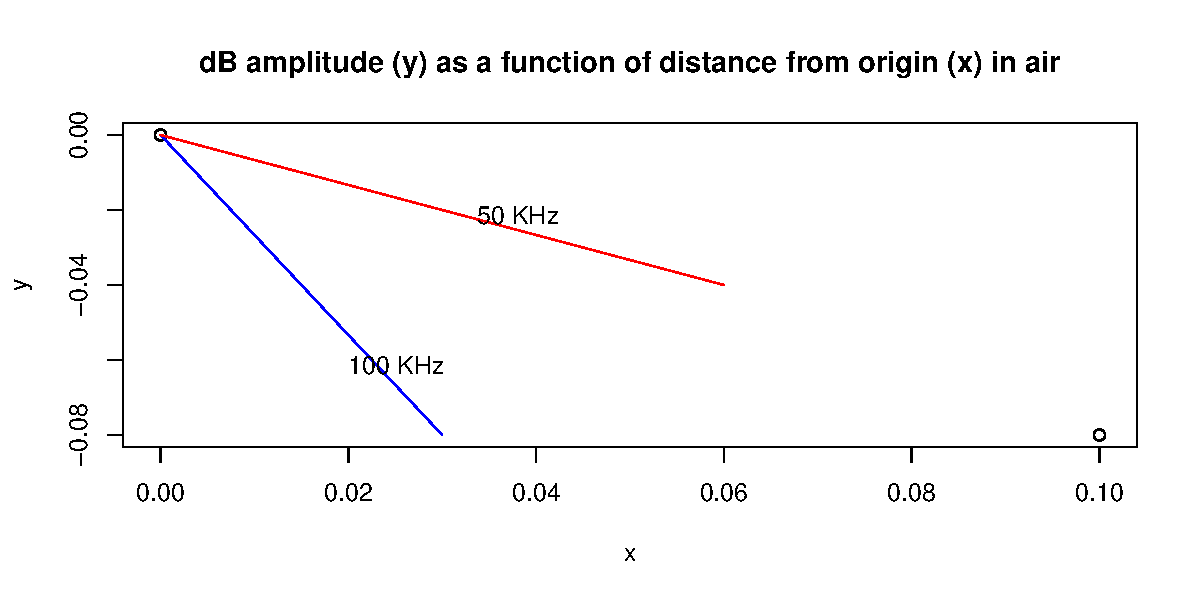
\includepdf[pages={1}]{air.pdf}
\end{document}
